\documentclass[cscoversheet,twoside]{i7-thesis}

\author{Simon Wittmann, Julian Kraus, Bastian Wiesner}

\germantitle{Green Epoch: Kohlenstoffbewusstes LLM-Training durch
Hysterese-Policy-Optimierung}
\title{Green Epoch: Carbon-Aware LLM Training via
Hysteresis Policy Optimization}

\course{Informatik}
\fakulty{Technische Fakultät}
\department{Department Computer Science}
\chair{Computer Science 7 - Computer Networks and Communication Systems}
\germandepartment{Department Informatik}
\germanchair{Lehrstuhl Informatik 7\\-\\Rechnernetze und Kommunikationssysteme}
\address{Martenstr.~3, 91058~Erlangen}
\website{https://www.cs7.tf.fau.de/}

\thesisend{21. May 2026}

\advisors{Prof.\ Dr-Ing. Reinhard German\newline Saeid Jahandar,
M.Sc.}

\watermarklogo{i7/watermark-inf.pdf}
\chairlogo{i7/i7-logo.pdf}
\faulogo{i7/techfak-logo.pdf}

\thesistype{Project Report}
\thesiscite{TODO}

\thesisstart{13. April 2026}

\usepackage{preamble}

\begin{document}
\maketitle
\pagenumbering{gobble}

%! TEX root = thesis.tex

\chapter*{Abstract}
\begin{otherlanguage*}{american}

The pretraining of large language models (LLMs) consumes millions of GPU-hours
and emits hundreds of tonnes of CO$_2$ per run.  Since grid carbon intensity
varies strongly over time and region, training can be paused during dirty
periods and resumed when the grid is cleaner.  We built a simulation framework
and an adaptive optimizer that searches over pause thresholds, resume
thresholds, and start dates to find the best configurations.  Using historical
electricity data at five-minute resolution, we evaluated two frontier
models---DeepSeek~V3 and Kimi~K2---across five regions with different grid
characteristics.  Our main finding is that the gap between pause and resume
threshold should be small (at most 16~gCO$_2$eq/kWh): a wide gap never pays
off.  In highly variable grids like Germany and Italy, savings reached 43\%
and 33\%, but came with up to 200\% longer training time.  In stable grids
like China and the US, savings stayed below 10\% regardless of the chosen
policy.  All code is implemented as a browser-based application with an
interactive simulator and optimizer, available as open source.

\end{otherlanguage*}

\chapter*{Kurzfassung}
\begin{otherlanguage*}{ngerman}

Das Pretraining gro{\ss}er Sprachmodelle (LLMs) verbraucht Millionen von
GPU-Stunden und emittiert hunderte Tonnen CO$_2$ pro Durchlauf.  Da die
CO$_2$-Intensit\"at des Stromnetzes stark \"uber Zeit und Region variiert,
l\"asst sich das Training in Zeiten hoher Emissionen pausieren und bei
saubererem Strom fortsetzen.  Wir haben eine Simulationsplattform und einen
adaptiven Optimierer entwickelt, der Pausenschwellen,
Fortsetzungsschwellen und Starttermine durchsucht, um die besten
Konfigurationen zu finden.  Anhand historischer Stromdaten in
F\"unf-Minuten-Aufl\"osung haben wir zwei Spitzenmodelle---DeepSeek~V3 und
Kimi~K2---in f\"unf Regionen mit unterschiedlichen Netzeigenschaften
evaluiert.  Unser wichtigstes Ergebnis: Der Abstand zwischen Pausen- und
Fortsetzungsschwelle sollte klein sein (maximal 16~gCO$_2$eq/kWh); ein gro{\ss}er
Abstand zahlt sich nie aus.  In stark variablen Netzen wie Deutschland und
Italien erreichten wir Einsparungen von 43\% bzw. 33\%, allerdings bei bis zu
200\% l\"angerer Trainingsdauer.  In stabilen Netzen wie China und den USA
blieben die Einsparungen unabh\"angig von der gew\"ahlten Strategie unter
10\%.  Der gesamte Code ist als browserbasierte Anwendung mit interaktivem
Simulator und Optimierer implementiert und als Open Source verf\"ugbar.

\end{otherlanguage*}

\cleardoublepage{}

\tableofcontents
\cleardoublepage{}

\pagenumbering{arabic}
\DTMsetdatestyle{iso}

%! TEX root = thesis.tex

\chapter{Introduction}
\label{sec:introduction}

The energy consumption of large language model (LLM) training has grown
dramatically. Training a single frontier model requires millions of GPU-hours
across thousands of accelerators: DeepSeek~V3 consumes 2.79M GPU-hours on 2048
H800 GPUs~\cite{deepseek-ai_deepseek-v3_2024} and Kimi~K2 trains on 15.5T
tokens with a minimum 256-GPU model-parallel group~\cite{kimi_team_kimi_2025}.
At a per-GPU power draw of 700~W and a power usage effectiveness of
1.27~\cite{jegham_hungry_2025}, a single run can emit hundreds of tonnes of
CO$_2$ depending on the local grid mix. As LLM deployment scales, managing
this environmental cost becomes essential for sustainable AI infrastructure.

Carbon-aware temporal workload shifting pauses training when grid carbon
intensity exceeds a threshold and resumes when it falls below a second
threshold. This approach allows a training run to consume cleaner energy
without hardware modification, but the threshold pair $(\theta_p, \theta_r)$
and start date $t_s$ jointly determine the savings-overhead trade-off. Prior
work on temporal shifting for cloud batch jobs reports 3--34\% operational
carbon savings~\cite{wiesner_lets_2021}, and geo-distributed training during
renewable curtailment windows achieves 88--95\% savings across multiple
sites~\cite{wiesner_distributed_2026}. However, none of these works provides a
systematic method for optimizing the hysteresis policy parameters of a
single-site LLM training run. Ad-hoc thresholds predominate, and the value of
the hysteresis margin (the gap between pause and resume thresholds) remains
unexplored.

We address this gap with a discrete-event simulation engine and an adaptive
grid-search optimizer that together search the three-dimensional policy space
$(\theta_p, \theta_r, t_s)$ and return Pareto-optimal configurations. The
optimizer converges within five to six iterations, requiring only
approximately 3,500 simulations per full optimization run (under one minute on
a single CPU core). We evaluate across two state-of-the-art models and five
electricity grid regions using 5-minute-resolution 2025 carbon intensity data
from Electricity Maps. Across tens of thousands of simulation runs, we
establish systematic Pareto frontiers for carbon-aware LLM training with
hysteresis-based pausing.

The results reveal a clear and actionable pattern: the optimal hysteresis
margin is consistently narrow ($\leq 16$~gCO$_2$eq/kWh), and wide hysteresis
degrades the savings-to-overhead ratio in every region and model
configuration. In high-variability grids (Germany, Italy), savings reach
43.4\% and 32.7\% at 174\% and 199\% time overhead. In low-variance grids
(China, United States), savings remain below 10\% regardless of the chosen
policy.

All simulation and optimization code is implemented as a fully client-side
browser application built with SolidJS and TypeScript, with no backend
dependency. The application provides an interactive live simulator, a batch
run dashboard, and an adaptive optimization page with 3D visualization of the
policy space. The complete project is available as open source.

This report is structured as follows. Chapter~\ref{sec:fundamentals} introduces
the necessary background on LLM training, grid carbon intensity, and hysteresis
policies. Chapter~\ref{sec:related_work} surveys related work in carbon-aware
computing. Chapter~\ref{sec:methodology} describes the simulation engine,
policy formulation, scoring, and optimization algorithm.
Chapter~\ref{sec:implementation} presents the software architecture and
implementation. Chapter~\ref{sec:experimental_setup} details the experimental
configuration. Chapter~\ref{sec:results} presents the full results.
Chapter~\ref{sec:validation_verification} describes validation and verification
procedures. Chapter~\ref{sec:conclusion} concludes with a summary of findings
and future work.

%! TEX root = thesis.tex

\chapter{Fundamentals}
\label{sec:fundamentals}

\section{LLM Pretraining}
\label{sec:llm-pretraining}

Large language models are neural networks with hundreds of billions of
parameters trained on trillions of text tokens.  The pretraining phase
dominates the total energy budget of an LLM lifecycle: it runs for weeks to
months on large GPU clusters.  For example, DeepSeek~V3, a 671B-parameter
mixture-of-experts model, required 2.79M GPU-hours on 2048 NVIDIA H800
GPUs~\cite{deepseek-ai_deepseek-v3_2024}.  Kimi~K2, a 1T-parameter mixture-of-experts model,
was trained on 15.5T tokens with a minimum 256-GPU model-parallel
group~\cite{kimi_team_kimi_2025}.  The effective energy consumption depends on
the GPU count, per-GPU power draw, and data center power usage effectiveness.

The training process is iterative: each step processes a batch of tokens,
computes gradients, and updates model weights.  This inherent repetitiveness
makes training amenable to pausing at natural breakpoints such as epoch
boundaries or checkpoints.  Modern training frameworks support asynchronous
checkpointing, which reduces the time overhead of saving and restoring model
state.

\section{Grid Carbon Intensity}
\label{sec:grid-carbon-intensity}

The carbon intensity of electricity measures the mass of CO$_2$ emitted per
unit of electrical energy consumed, typically expressed in
gCO$_2$eq/kWh.  Grid carbon intensity varies on multiple timescales:
\begin{itemize}
  \item \textbf{Hourly}: solar generation causes midday dips on sunny days;
    wind patterns create overnight fluctuations.
  \item \textbf{Daily}: weekday vs.\ weekend demand patterns shift the generation
    mix.
  \item \textbf{Seasonal}: winter heating demand and summer cooling demand
    alter the marginal generator.
  \item \textbf{Regional}: grids with high renewable penetration (e.g., Sweden)
    have low mean intensity; grids reliant on coal (e.g., China) have high
    mean intensity.
\end{itemize}

These variations create opportunities for temporal workload shifting.  A
training job running in Germany in 2025 experiences a mean intensity of
approximately 380~gCO$_2$eq/kWh with a standard deviation of 142~gCO$_2$eq/kWh
(coefficient of variation 0.37).  This wide range means periods of
near-zero-carbon power alternate with fossil-dominated intervals, making
Germany a promising candidate for carbon-aware scheduling.  In contrast, the
Chinese grid averages 519~gCO$_2$eq/kWh with low variability (coefficient of variation 0.11),
offering few clean intervals worth waiting for.

Carbon intensity data is available from services such as Electricity Maps,
which provides historical and fore-casted marginal intensity at 5-minute
resolution for most global regions.  Marginal intensity (the intensity of the
generator on the margin) is more appropriate for assessing the impact of an
additional load than average intensity~\cite{dodge_measuring_2022}.

\section{Temporal Workload Shifting}
\label{sec:temporal-workload-shifting}

Temporal workload shifting delays or pauses computational workloads during
periods of high grid carbon intensity and resumes them when the grid is
cleaner.  The core trade-off is between carbon savings (reduced operational
emissions) and time overhead (extended wall-clock duration).  The approach
requires no hardware modification and is applicable to any interruptible
workload with checkpointing support.

Prior work has applied temporal shifting to generic cloud batch
jobs~\cite{wiesner_lets_2021}, achieving 3--34\% operational carbon savings
depending on the delay tolerance and regional grid characteristics.  For LLM
training, the savings potential depends on model scale (larger GPU clusters
consume more power per unit time, increasing the absolute benefit of pausing),
checkpoint overhead (frequent saving and restoring adds time and energy), and
grid variability (high-variance grids offer more arbitrage opportunities).

\section{Hysteresis}
\label{sec:hysteresis}

A hysteresis policy uses separate thresholds for entering and leaving a state
to prevent rapid toggling.  In the context of carbon-aware training, two
thresholds define the policy:
\begin{itemize}
  \item $\theta_p$: the pause threshold.  When training is active and carbon
    intensity exceeds $\theta_p$, training pauses.
  \item $\theta_r$: the resume threshold.  When paused and carbon intensity
    falls below $\theta_r$, training resumes.
\end{itemize}

The condition $\theta_r \le \theta_p$ must hold.  The difference $\Delta_\theta
= \theta_p - \theta_r$ is the hysteresis margin.  A margin of zero
($\theta_r = \theta_p$) means the job toggles at a single threshold.  For a
positive margin, intensities in the interval $[\theta_r, \theta_p]$ form a dead
zone where the job remains in its current state, preventing flutter---rapid
pause-resume cycles triggered by small fluctuations around a single threshold.

Hysteresis introduces a trade-off: a wider margin reduces the number of
transitions (saving checkpoint overhead) but also leaves the job paused through
moderately clean intervals that could have been exploited productively.
Identifying the optimal margin for a given region and model is the central
focus of this work.

%! TEX root = thesis.tex

\chapter{Related Work}
\label{sec:related_work}

\section{Temporal Workload Shifting}

Temporal workload shifting delays computational jobs to align with periods of
low grid carbon intensity.  Wiesner~et~al.~\cite{wiesner_lets_2021}
demonstrated that delaying cloud batch jobs by a few hours can reduce
operational emissions by 3--34\%, with negligible checkpoint overhead enabling
higher savings.  Their work uses a single threshold for pause decisions and
does not explore hysteresis.  Carbon Explorer~\cite{acun_carbon_2023} balances
operational and embodied carbon at the datacenter planning timescale, but
operates at the level of hardware procurement and deployment decisions rather
than per-run scheduling.

\section{Carbon-Aware Distributed Training}

Extending temporal shifting to geo-distributed training adds spatial
flexibility.  Wiesner~et~al.~\cite{wiesner_distributed_2026} trained a
561M-parameter transformer across multiple sites during renewable curtailment
windows, reducing emissions to 5--12\% of the baseline.  Their approach
exploits near-zero-carbon curtailment energy but requires multiple
geographically distributed data centers.  Our work complements this by
optimizing the hysteresis policy for single-site training, which is the more
common deployment scenario.

\section{Emissions Accounting Methodology}

Accurate carbon accounting is essential for evaluating the savings from
temporal shifting.  Patterson~et~al.~\cite{patterson_carbon_nodate} propose a
methodology based on GPU-hours, thermal design power, power usage effectiveness, and grid intensity.
Dodge~et~al.~\cite{dodge_measuring_2022} highlight the importance of using
marginal rather than average grid intensity, and demonstrate that
time-specific cloud data yields more accurate estimates.  We follow their
recommendation by using marginal carbon intensity at 5-minute resolution.



%! TEX root = thesis.tex

\chapter{Methodology}
\label{sec:methodology}

\section{System Model}
\label{sec:system-model}

We model a single training job defined by: model parameter count $N$, dataset
token count $T$, GPU count $G$, per-GPU training power $P_t$, per-GPU idle
power $P_i$, facility power usage effectiveness $\eta$, checkpoint save duration $\tau_c$, and
checkpoint resume duration $\tau_r$.  The job runs on a cluster in a single
region whose grid carbon intensity $c(t)$ is given as a time series at
5-minute resolution.

The baseline (never-pause) scenario runs the job uninterrupted.  Total
baseline energy is
\[
E_b = G \cdot P_t \cdot \eta \cdot T_b
\]
where $T_b$ is the baseline training duration derived from $T$ tokens,
GPU-hours, and $G$.  Baseline emissions are $E_b \cdot \bar{c}$, where
$\bar{c}$ is the time-averaged carbon intensity over the training window.

\section{Discrete-Event Simulator}
\label{sec:simulator}

The core of our framework is a discrete-event simulator that replays a
training run under a given policy.  At each 5-minute timestep $\Delta t$, the
simulator:
\begin{itemize}
  \item Checks the current state (training or paused).
  \item Applies the hysteresis policy to determine whether to switch state.
  \item Computes energy consumption based on the active or idle GPU power.
  \item Computes emissions as energy multiplied by the current grid carbon
    intensity.
  \item Tracks training progress as fraction of total tokens completed.
\end{itemize}

When a pause is triggered, the simulator adds a checkpoint save duration
$\tau_c$ at full GPU power before entering idle state.  When a resume is
triggered, it adds a checkpoint load duration $\tau_r$ (typically negligible
with asynchronous checkpointing).  The simulation terminates when training
progress reaches 100\%.

Energy per timestep is
\[
E(t) = G \cdot P \cdot \eta \cdot \Delta t
\]
where $P = P_t$ when training and $P = P_i$ when paused.  Emissions are
$E(t) \cdot c(t)$.  Total wall-clock time includes both active training time
and paused intervals including checkpoint overhead.

Figure~\ref{fig:grid-replay} visualizes this core grid-replay loop as an activity diagram.

\begin{figure}
  \centering
  
\includegraphics[width=0.6\textwidth]{figures/activity_grid_replay}
  \caption{Grid-replay loop of the simulation engine. At each timestep the
  simulator reads the current carbon intensity, evaluates the hysteresis policy
  to decide whether to pause or resume, and accumulates energy, emissions, and
  wall-clock time accordingly.}
  \label{fig:grid-replay}
\end{figure}

\section{Hysteresis Policy}
\label{sec:hysteresis-policy}

A policy $\pi$ is defined by the triple $(\theta_p, \theta_r, t_s)$:
\begin{itemize}
  \item $\theta_p$ (gCO$_2$eq/kWh): pause threshold.  When training and
    $c(t) > \theta_p$, training pauses.
  \item $\theta_r$ (gCO$_2$eq/kWh): resume threshold.  When paused and
    $c(t) \le \theta_r$, training resumes.
  \item $t_s$ (datetime): start date and time of the training run.
\end{itemize}

The policy is feasible only if $\theta_r \le \theta_p$.  The hysteresis margin
$\Delta_\theta = \theta_p - \theta_r$ controls the width of the dead zone.

\section{Scoring of Policies}
\label{sec:scoring}

Policies are evaluated against the never-pause baseline using two primary
key performance indicators:
\begin{align*}
  \text{CO2\_savings\_pct} &= \frac{E_b - E_p}{E_b} \times 100, \\
  \text{time\_overhead\_pct} &= \frac{T_p - T_b}{T_b} \times 100,
\end{align*}
where $E_b, T_b$ are baseline energy and time, and $E_p, T_p$ are policy
energy and time.

For ranking policies, we use a composite score that rewards carbon savings
while enforcing a hard overhead budget $B$:
\[
\text{score} = \frac{
  \alpha \cdot \frac{\text{CO2\_savings\_pct}}{100}
  + (1-\alpha) \cdot \left(1 - \frac{\text{time\_overhead\_pct}}{B}\right)
}{2}
\]
with feasibility constraint $\text{time\_overhead\_pct} \le B$.  The
parameter $\alpha \in [0,1]$ controls the trade-off between savings
maximization and overhead minimization.  In all experiments reported here, we
use $\alpha = 1$, which simplifies the score to $\frac{1}{2} +
\frac{\text{CO2\_savings\_pct}}{200}$---pure savings maximization subject to
the overhead budget.  The never-pause baseline has score 0.5.

\section{Adaptive Grid-Search Optimization}
\label{sec:optimization}

Exhaustively enumerating the three-dimensional policy space $(\theta_p,
\theta_r, t_s)$ is computationally prohibitive.  A naive grid at resolution
$N$ per axis costs $O(N^2 \cdot D)$ simulations, where $D$ is the number of
start-date samples.  With $N=100$ and $D=52$, brute-force would require
approximately 260,000 simulations.

We instead use an adaptive grid-search algorithm inspired by trust-region
optimization:
\begin{enumerate}
  \item \textbf{Initialization.} A coarse grid over full bounds:
    $\theta_p \in [0, \theta_p^{\max}]$, $\theta_r \in [0, \theta_p]$, and
    $t_s$ at $D$ uniform intervals.  The maximum $\theta_p^{\max}$ is
    region-dependent: 100~gCO$_2$eq/kWh for Sweden (whose maximum intensity is
    low), 800 for all other regions.
  \item \textbf{Evaluation and selection.} Every grid point is simulated.
    Points exceeding the overhead budget $B$ are discarded.  From feasible
    points, the highest-scoring is selected.
  \item \textbf{Zoom refinement.} Bounds contract around the best point by a
    shrink factor $s = 0.45$ per axis.  Grid resolution remains fixed at
    $N = 10$ points per axis per iteration.  If the contracted interval on any
    axis falls below the minimum step of $3$~gCO$_2$eq/kWh, search on that
    axis terminates.
  \item \textbf{Iteration.} Steps 2--3 repeat for a maximum of $K = 10$
    iterations.  The shrink factor $s = 0.45$ ensures that after approximately
    six iterations the search window contracts below the minimum step.
\end{enumerate}

The algorithm guarantees a feasible point: the initial grid always contains the
zero-hysteresis no-pause policy $\theta_p = \theta_p^{\max}, \theta_r = 0$,
which yields 0\% overhead.  Total complexity is $O(K \cdot N^2 \cdot D)$.
With our settings ($K=10, N=10, D=7$ for start-date experiments, $D=1$ for
fixed-date runs), a full optimization evaluates approximately 3,500 candidate
policies (550 for fixed-start runs), completing in under one minute on a
single CPU core.  The optimizer converges within 5--6 iterations in all
(model, region) combinations; subsequent iterations yield no measurable
improvement.

\section{Carbon Intensity Data}
\label{sec:carbon-data}

Carbon intensity data is sourced from the Electricity Maps API at 5-minute
resolution.  Table~\ref{tab:grid} summarizes the statistical characteristics of
the five regions used in this study.  The regions span a wide range: Sweden
(clean, highly variable), Germany and Italy (moderately dirty, highly
variable), and the United States and China (moderate-to-dirty, low
variability).

\begin{table}
    \centering
    \caption{Grid carbon intensity characteristics (2025).  Regions ordered by
    coefficient of variation.}
    \label{tab:grid}
    \small
    \begin{tabular}{lrrr}
      \toprule
      Region & Mean & Std.\ dev. & Coeff.\ of var.\ \\
      & (gCO$_2$eq/kWh) & (gCO$_2$eq/kWh) & \\
      \midrule
      DE (Germany) & 380 & 141.98 & 0.37 \\
      SE (Sweden)  &  23 &   8.19 & 0.35 \\
      IT (Italy)   & 309 &  87.02 & 0.28 \\
      US (United States) & 412 & 44.68 & 0.11 \\
      CN (China)   & 519 &  55.68 & 0.11 \\
      \bottomrule
    \end{tabular}
\end{table}

Grid variability, not mean intensity, determines savings potential.  Germany
(coefficient of variation 0.37) and Italy (coefficient of variation 0.28) offer the greatest temporal arbitrage
opportunity because their carbon intensity oscillates between near-zero and
high values on hourly timescales.  Sweden has high relative variability (coefficient of variation
0.35) but such a low mean (23~gCO$_2$eq/kWh) that the absolute emissions
available to avoid are limited.  The United States and China (coefficient of variation 0.11) are
consistently moderate and consistently dirty, respectively, offering few clean
intervals worth waiting for.

The time series exhibits strong temporal autocorrelation (lag-1 correlation
0.999, one-day lag 0.694 for Germany), making chronological trace replay
essential over independent sampling.

%! TEX root = thesis.tex

\chapter{Software Architecture and Implementation}
\label{sec:implementation}

\section{Technology Stack}
\label{sec:tech-stack}

The Green Epoch application is implemented as a fully client-side single-page
application using SolidJS with TypeScript.  The entire simulation engine
and optimizer run in the browser; the server only serves static files.  This
architecture eliminates backend dependencies, reduces operational cost, and
makes the application accessible to anyone with a web browser.

\begin{itemize}
  \item \textbf{Frontend framework:} SolidJS 1.9 with reactive state
    management, compiled by Vite.
  \item \textbf{Styling:} Tailwind CSS 4 with dark and light mode support.
  \item \textbf{Charts:} Chart.js for time-series carbon intensity plots,
    Plotly for 3D scatter visualization of the optimization space.
  \item \textbf{Simulation:} Pure TypeScript domain logic, run inside Web
    Workers for non-blocking execution.
  \item \textbf{Testing:} Vitest with testing-library for component and
    unit tests.
  \item \textbf{CLI:} Commander.js-based command-line interface for headless
    simulation and optimization.
\end{itemize}

\section{Architecture Overview}
\label{sec:architecture}

The application follows a three-layer architecture that separates pure business
logic from execution and presentation:

\begin{description}
  \item[Domain layer:] Pure TypeScript modules with no UI or side-effect
    dependencies.  Contains the simulation step engine, physics constants,
    hysteresis policy, scoring functions, and the adaptive grid-search
    optimizer.  This layer is fully portable and is also used by the CLI.
  \item[Engine layer:] Web Worker wrappers that offload simulation,
    optimization, batch runs, and CO$_2$ data loading to background threads.
    Each worker communicates with the UI via message passing, posting progress
    updates and results asynchronously.
  \item[UI layer:] SolidJS page components implementing the four main views:
    scenarios overview, single-run simulation, batch run dashboard, and
    optimization page.  Reusable components include the CO$_2$ time-series
    chart, stats panels, scenario forms, and the 3D optimization plot.
\end{description}

Figure~\ref{fig:scenarios-overview} shows the scenarios overview page where users manage their simulation configurations.

\begin{figure}
  \centering
  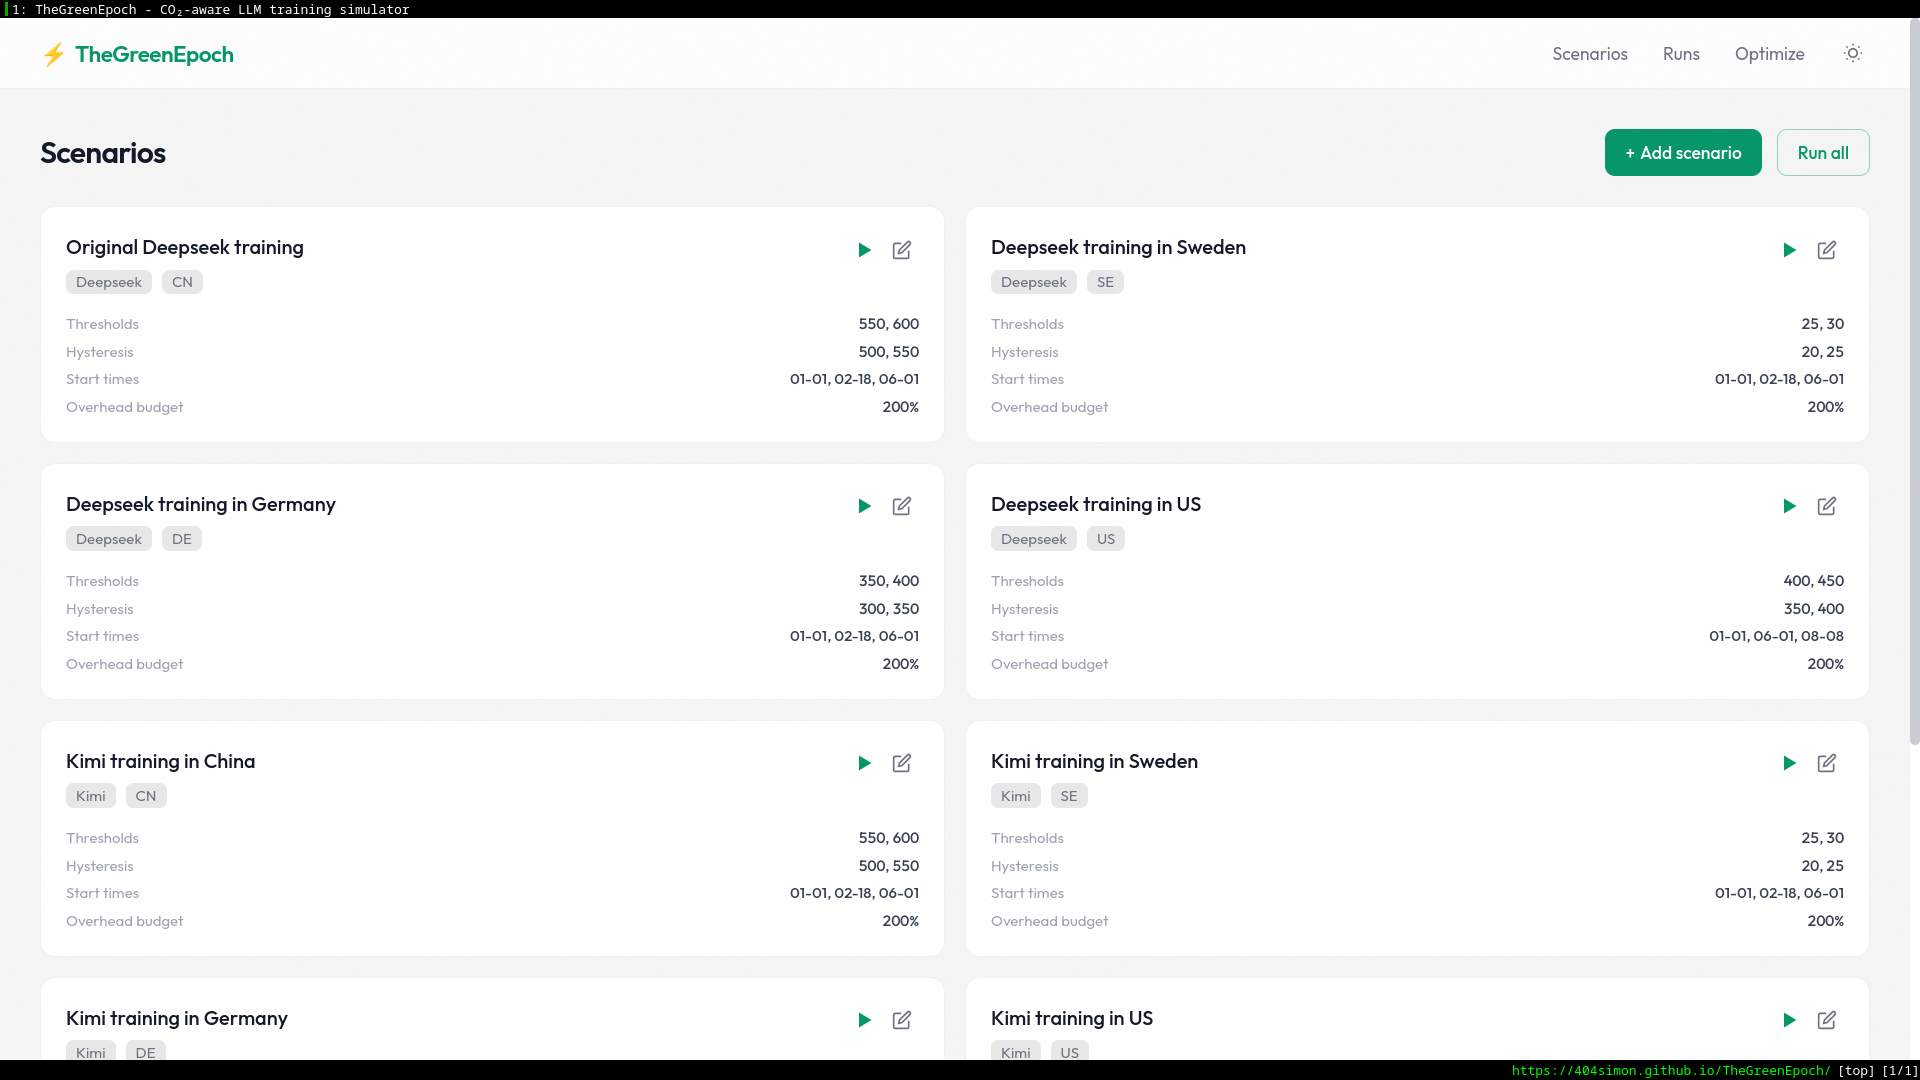
\includegraphics[width=\textwidth]{figures/screenshots/scenarios_overview_page}
  \caption{Scenarios overview page: users can view, create, edit, and launch
  simulation scenarios.}
  \label{fig:scenarios-overview}
\end{figure}

\section{Simulation Engine}
\label{sec:simulation-engine}

The simulation engine is the core of the domain layer.  It exposes a single
generator function \texttt{simulateStepwise()} that yields simulation state
at each timestep.  This design enables both real-time visualization (by
consuming the generator incrementally) and batch execution (by draining it to
completion).

Key design decisions include:
\begin{itemize}
  \item \textbf{Timestep alignment.} The CO$_2$ timeline is indexed by Unix
    timestamp.  The simulator advances through the timeline in 5-minute steps,
    querying the current intensity via binary search.
  \item \textbf{State machine.} The pause/resume logic is implemented as a
    deterministic finite state machine with four states: training, pausing
    (checkpoint save), paused, and resuming (checkpoint load).
  \item \textbf{Progress accounting.} Training progress increments only during
    the training state.  Baseline duration is computed from the training
    profile (tokens, GPU-hours, GPU count).  Wall-clock time accumulates
    across all states.
\end{itemize}

The interactive simulation view is shown in Figure~\ref{fig:single-run-top}, which displays the CO$_2$ intensity chart with threshold annotations and real-time KPIs. Figure~\ref{fig:single-run-bottom} presents the detailed comparison against the never-pause baseline below the chart area.

\begin{figure}
  \centering
  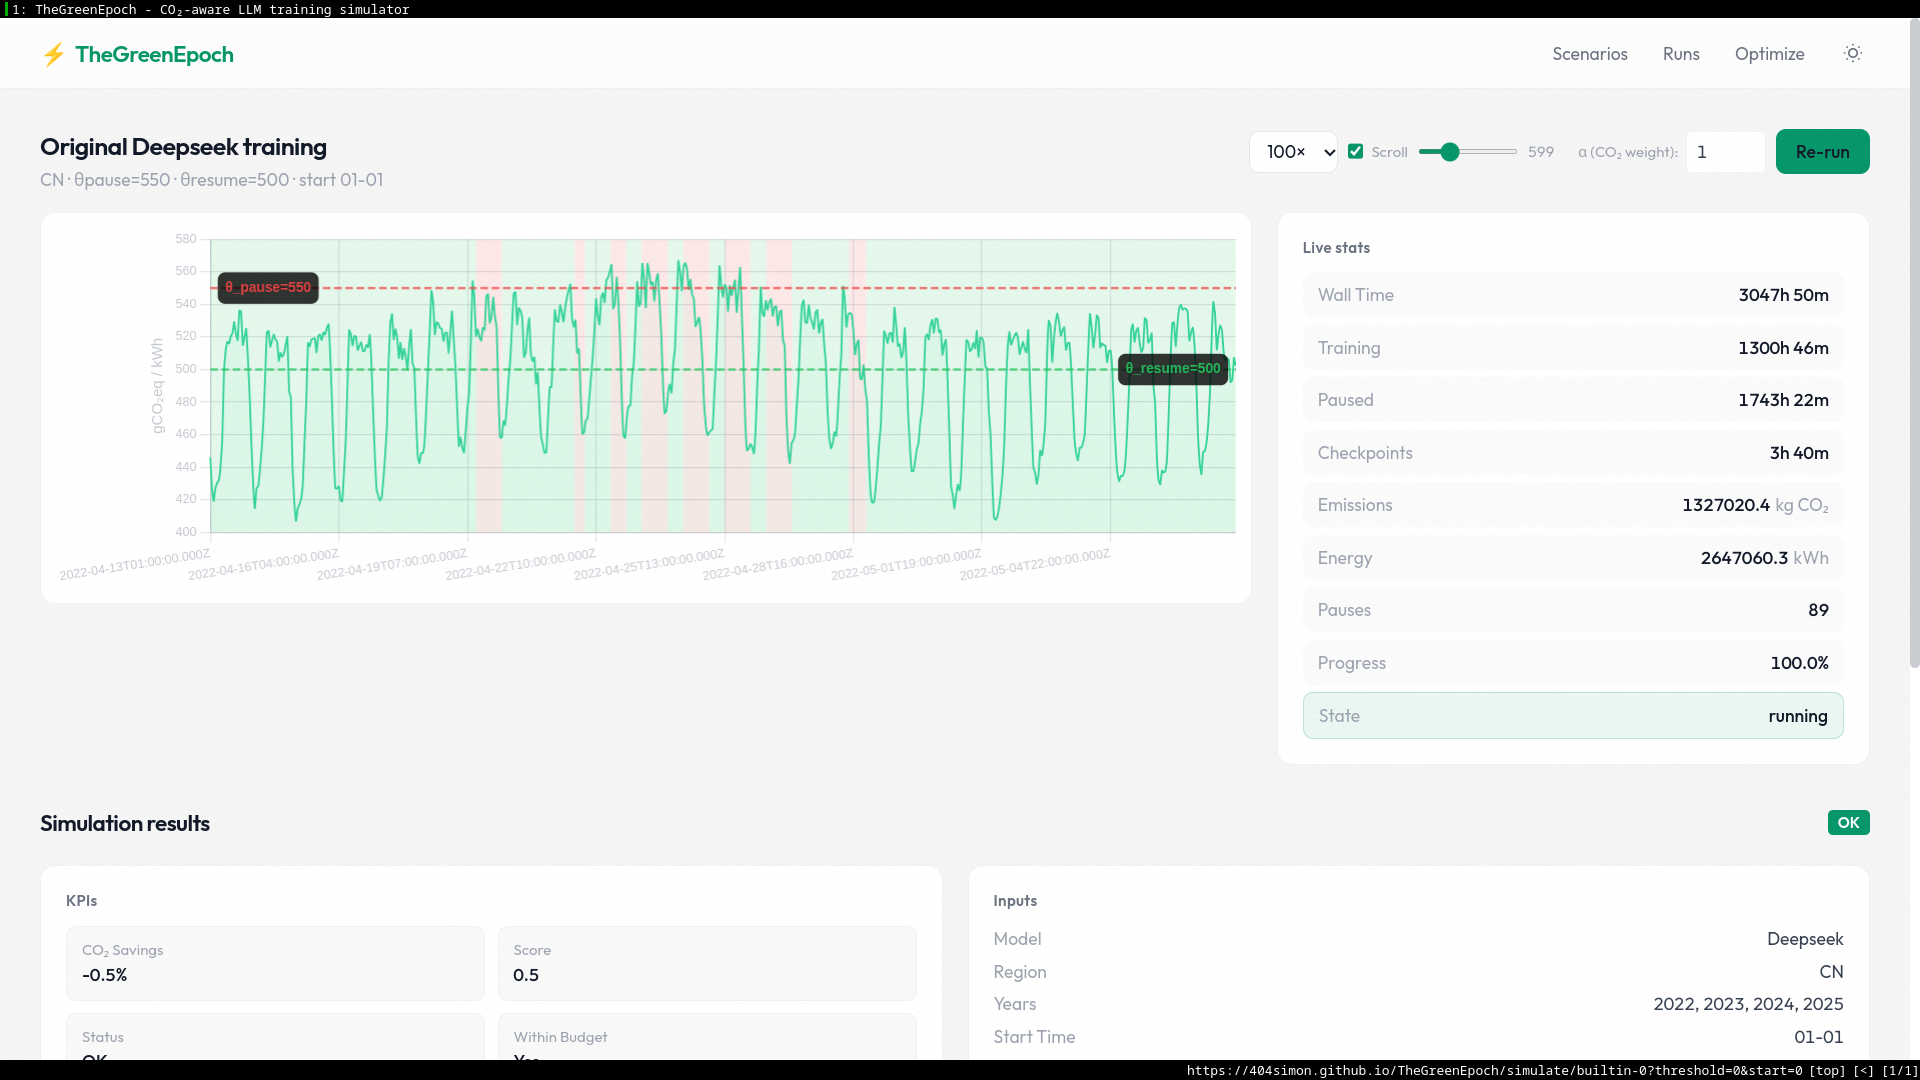
\includegraphics[width=\textwidth]{figures/screenshots/single_scenario_run_top_page}
  \caption{Single scenario run view: interactive simulation with CO$_2$
  intensity chart, pause/resume threshold annotations, and real-time
  statistics.}
  \label{fig:single-run-top}
\end{figure}

\begin{figure}
  \centering
  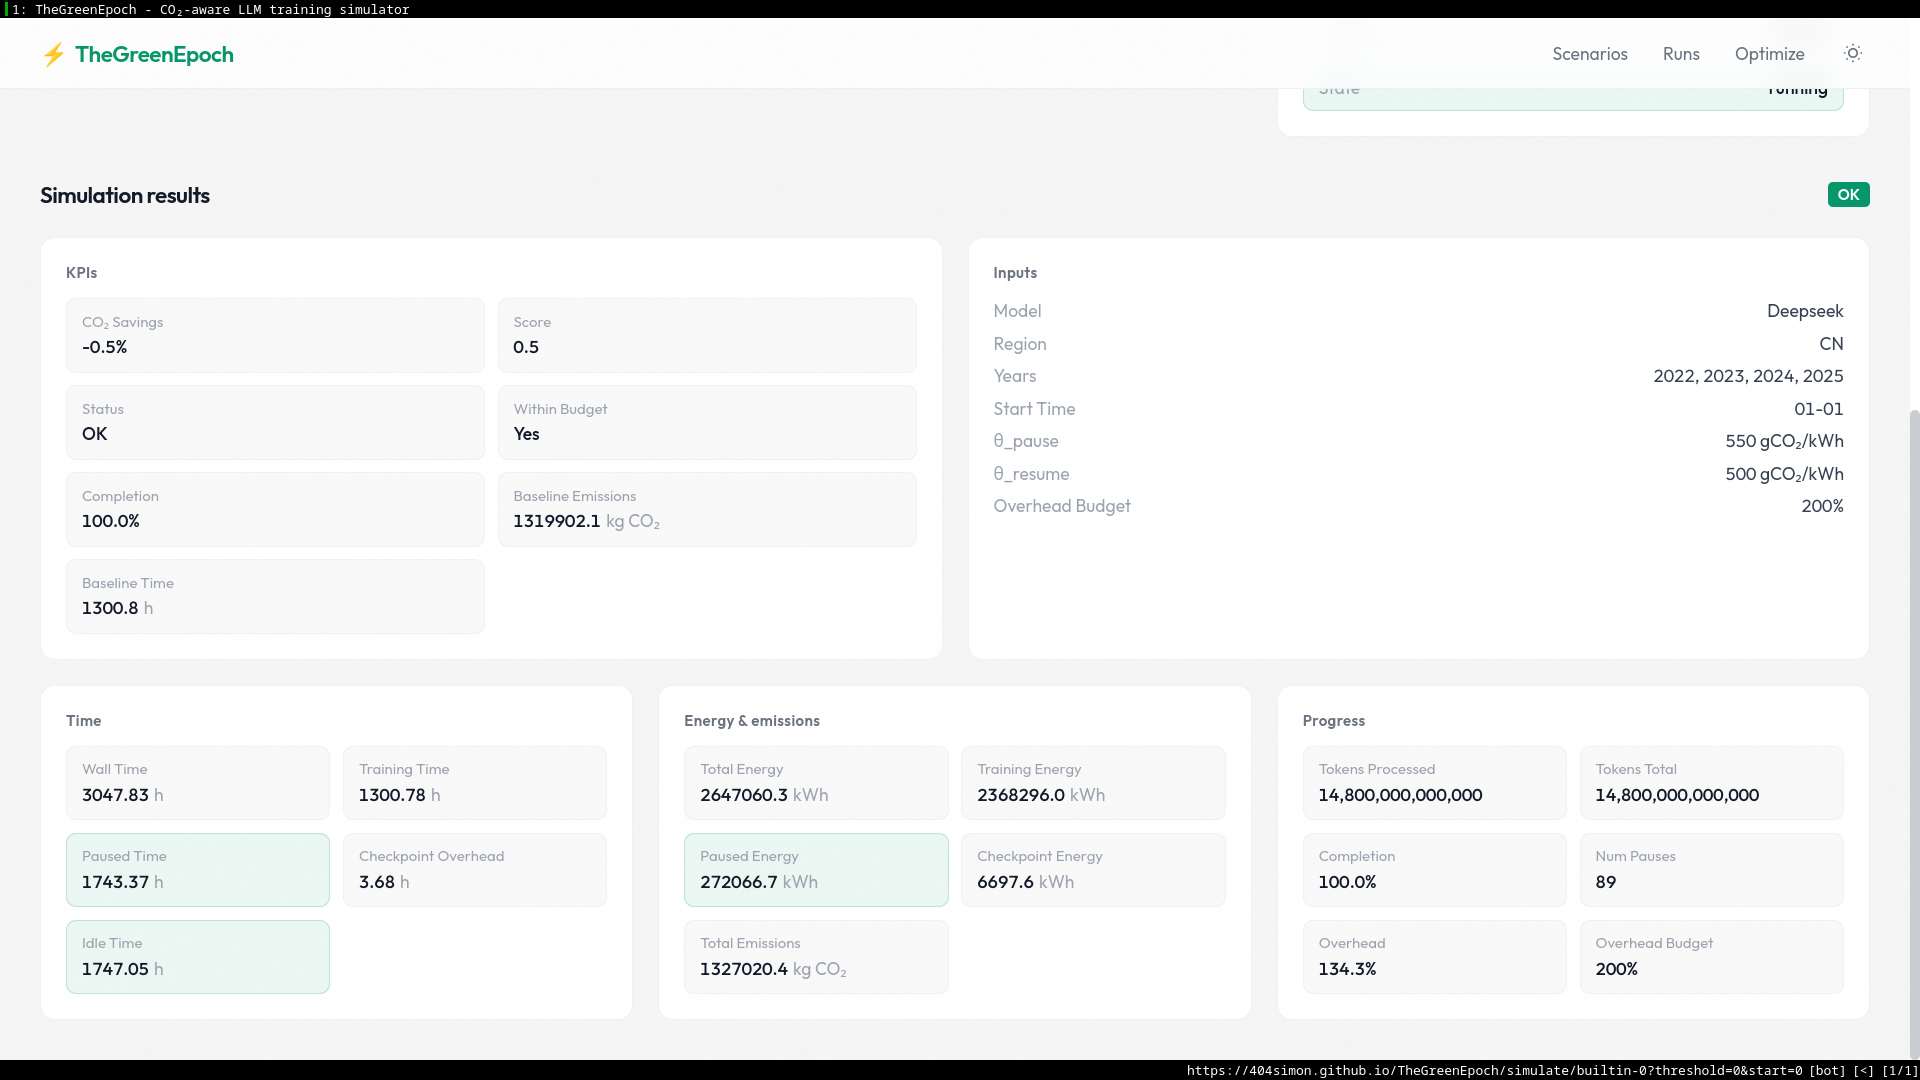
\includegraphics[width=\textwidth]{figures/screenshots/single_scenario_run_bottom_page}
  \caption{Single scenario run view (bottom): detailed KPIs comparing policy
  results against the never-pause baseline.}
  \label{fig:single-run-bottom}
\end{figure}

\section{Adaptive Optimizer}
\label{sec:optimizer-implementation}

The adaptive grid-search optimizer is implemented as a Web Worker that runs
iterations asynchronously.  Each iteration:
\begin{enumerate}
  \item Generates a grid of $(\theta_p, \theta_r, t_s)$ samples at the current
    resolution.
  \item Spawns individual simulation calls for each grid point.
  \item Collects results, scores them, and identifies the best point.
  \item Contracts the search bounds and reports progress to the UI.
\end{enumerate}

The optimizer posts \texttt{iteration} events after each zoom step, allowing
the UI to render intermediate results.  This gives the user real-time feedback
on convergence.

Figure~\ref{fig:optim-settings} shows the optimizer configuration panel where model, region, and algorithm parameters are selected. The resulting three-dimensional policy space is visualized in Figure~\ref{fig:optim-3d} as a color-coded scatter plot.

\begin{figure}
  \centering
  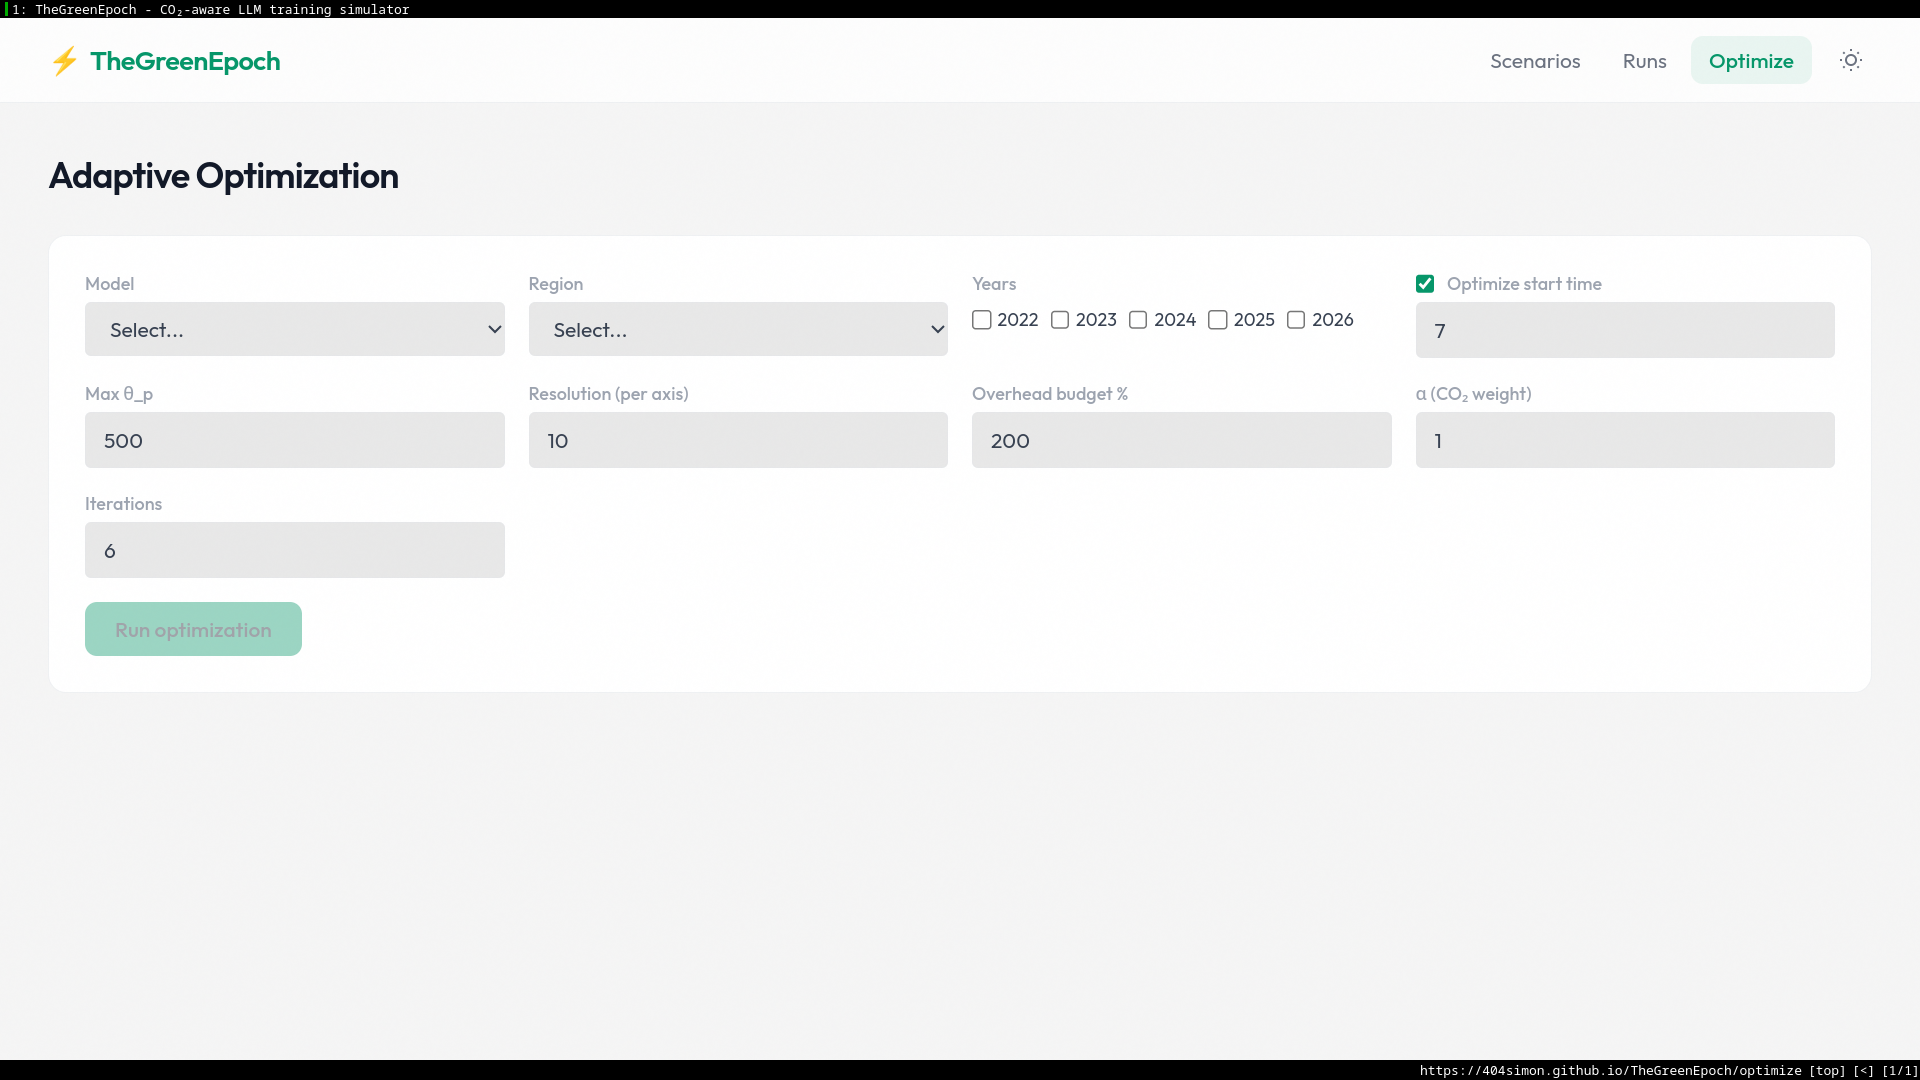
\includegraphics[width=\textwidth]{figures/screenshots/adaptive_optimization_page_settings}
  \caption{Optimization page settings panel: select model, region, years, and
  optimizer parameters.}
  \label{fig:optim-settings}
\end{figure}

\begin{figure}
  \centering
  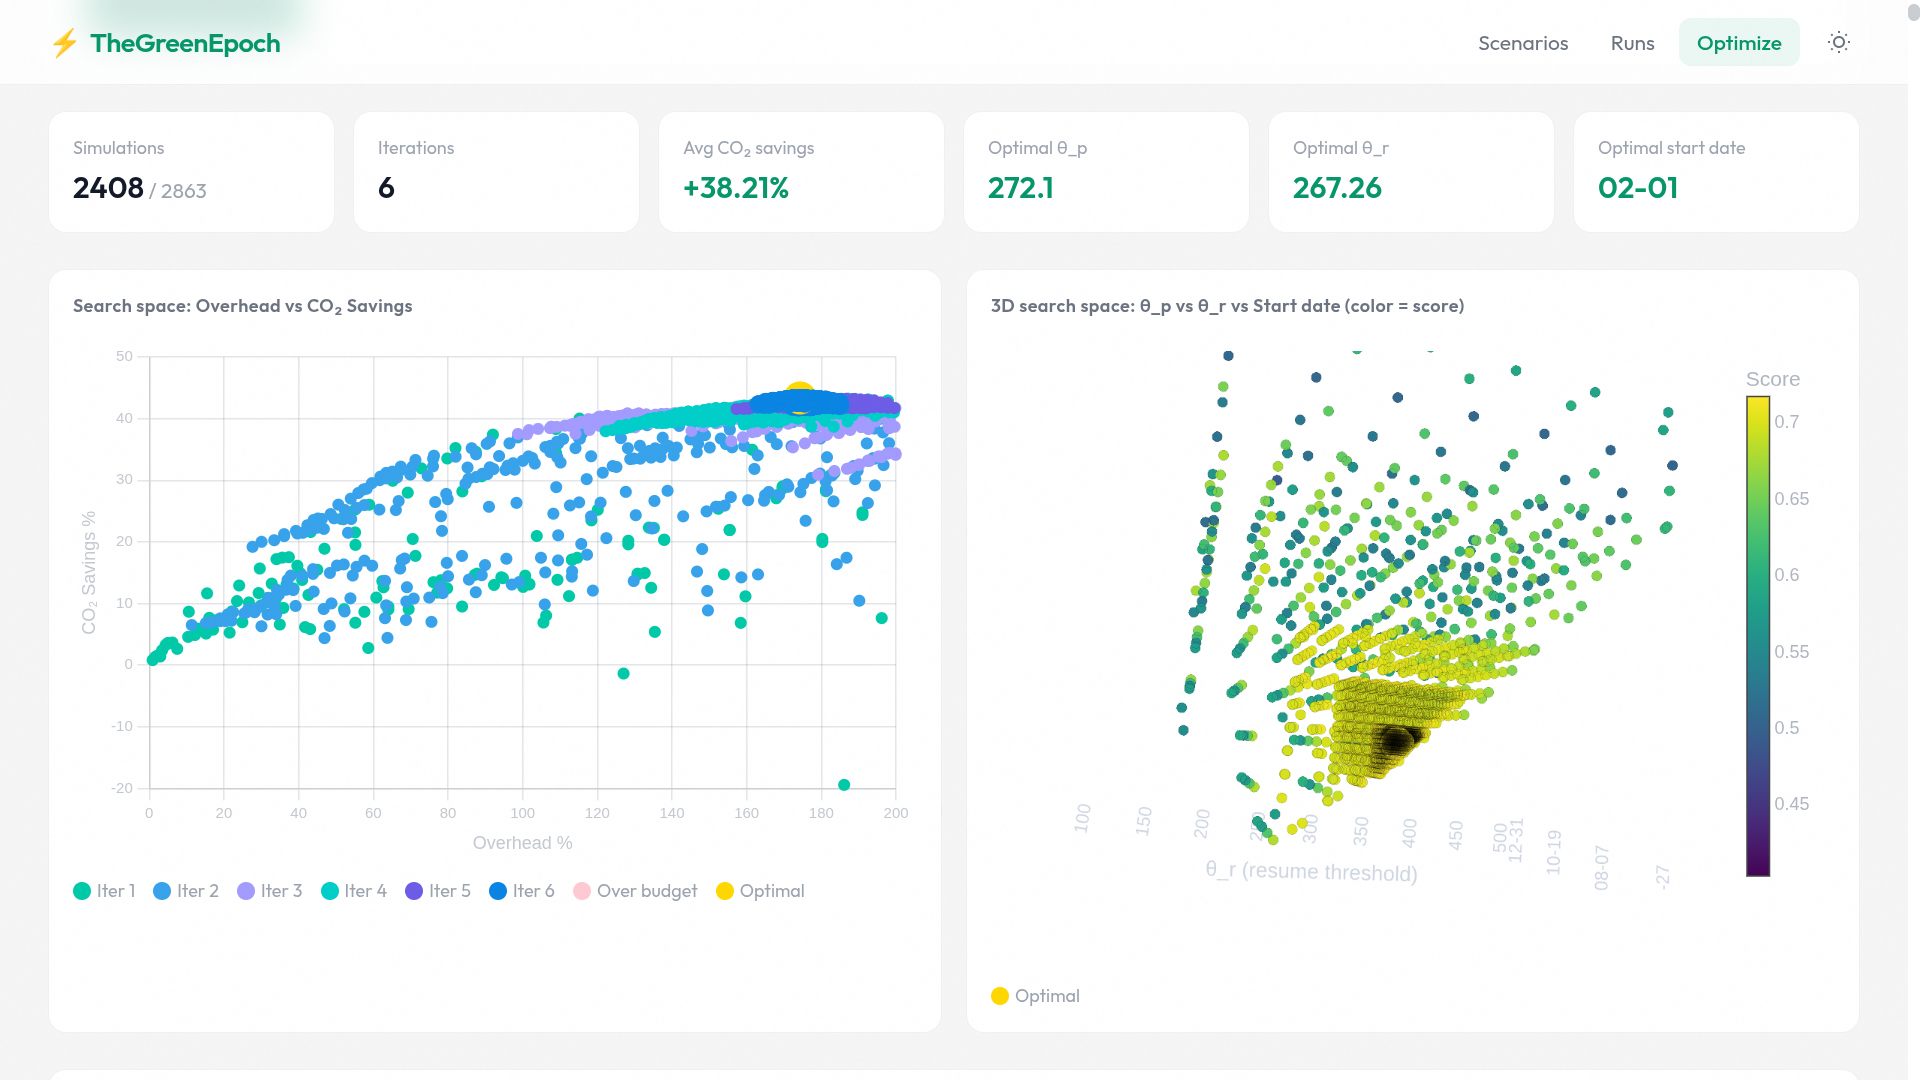
\includegraphics[width=\textwidth]{figures/screenshots/adaptive_optimization_page_results_middle_page_2}
  \caption{Optimization results: 3D scatter plot of pause threshold vs.\
  resume threshold vs.\ start date, colored by score.}
  \label{fig:optim-3d}
\end{figure}

\section{Batch Run Dashboard}
\label{sec:batch-dashboard}

The batch run page executes all configured scenarios across their threshold
and start-time combinations.  Results are displayed in a scatter plot
(overhead vs.\ CO$_2$ savings) and a sortable, filterable results table.  The
batch runner uses a dedicated Web Worker that processes scenarios sequentially
and posts results back progressively, providing a live progress indicator
(Figure~\ref{fig:batch-progress}). After completion, the scatter plot
(Figure~\ref{fig:batch-scatter}) visualizes the savings-overhead trade-off
across all evaluated configurations, and the sortable results table
(Figure~\ref{fig:batch-table}) provides detailed per-policy metrics.

\begin{figure}
  \centering
  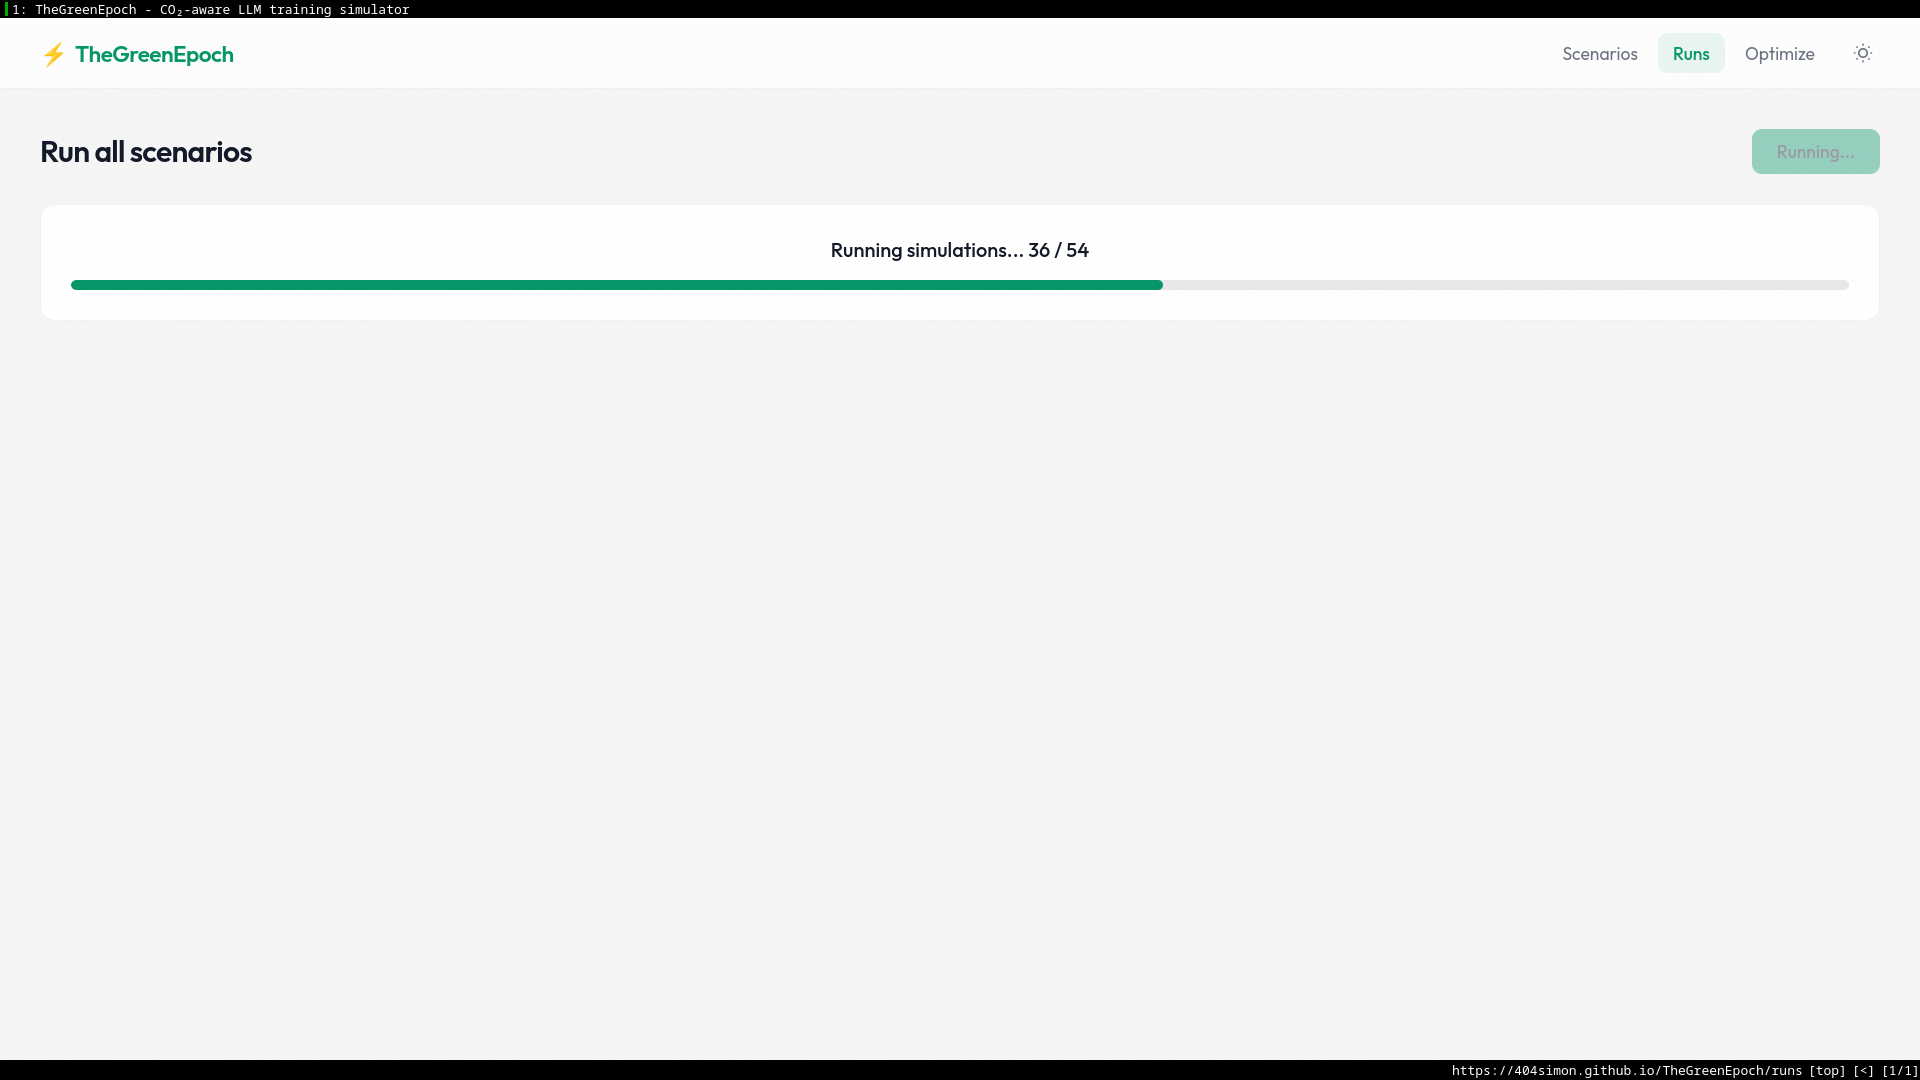
\includegraphics[width=\textwidth]{figures/screenshots/run_all_page_progress}
  \caption{Batch run dashboard showing progress and partial results during
  execution.}
  \label{fig:batch-progress}
\end{figure}

\begin{figure}
  \centering
  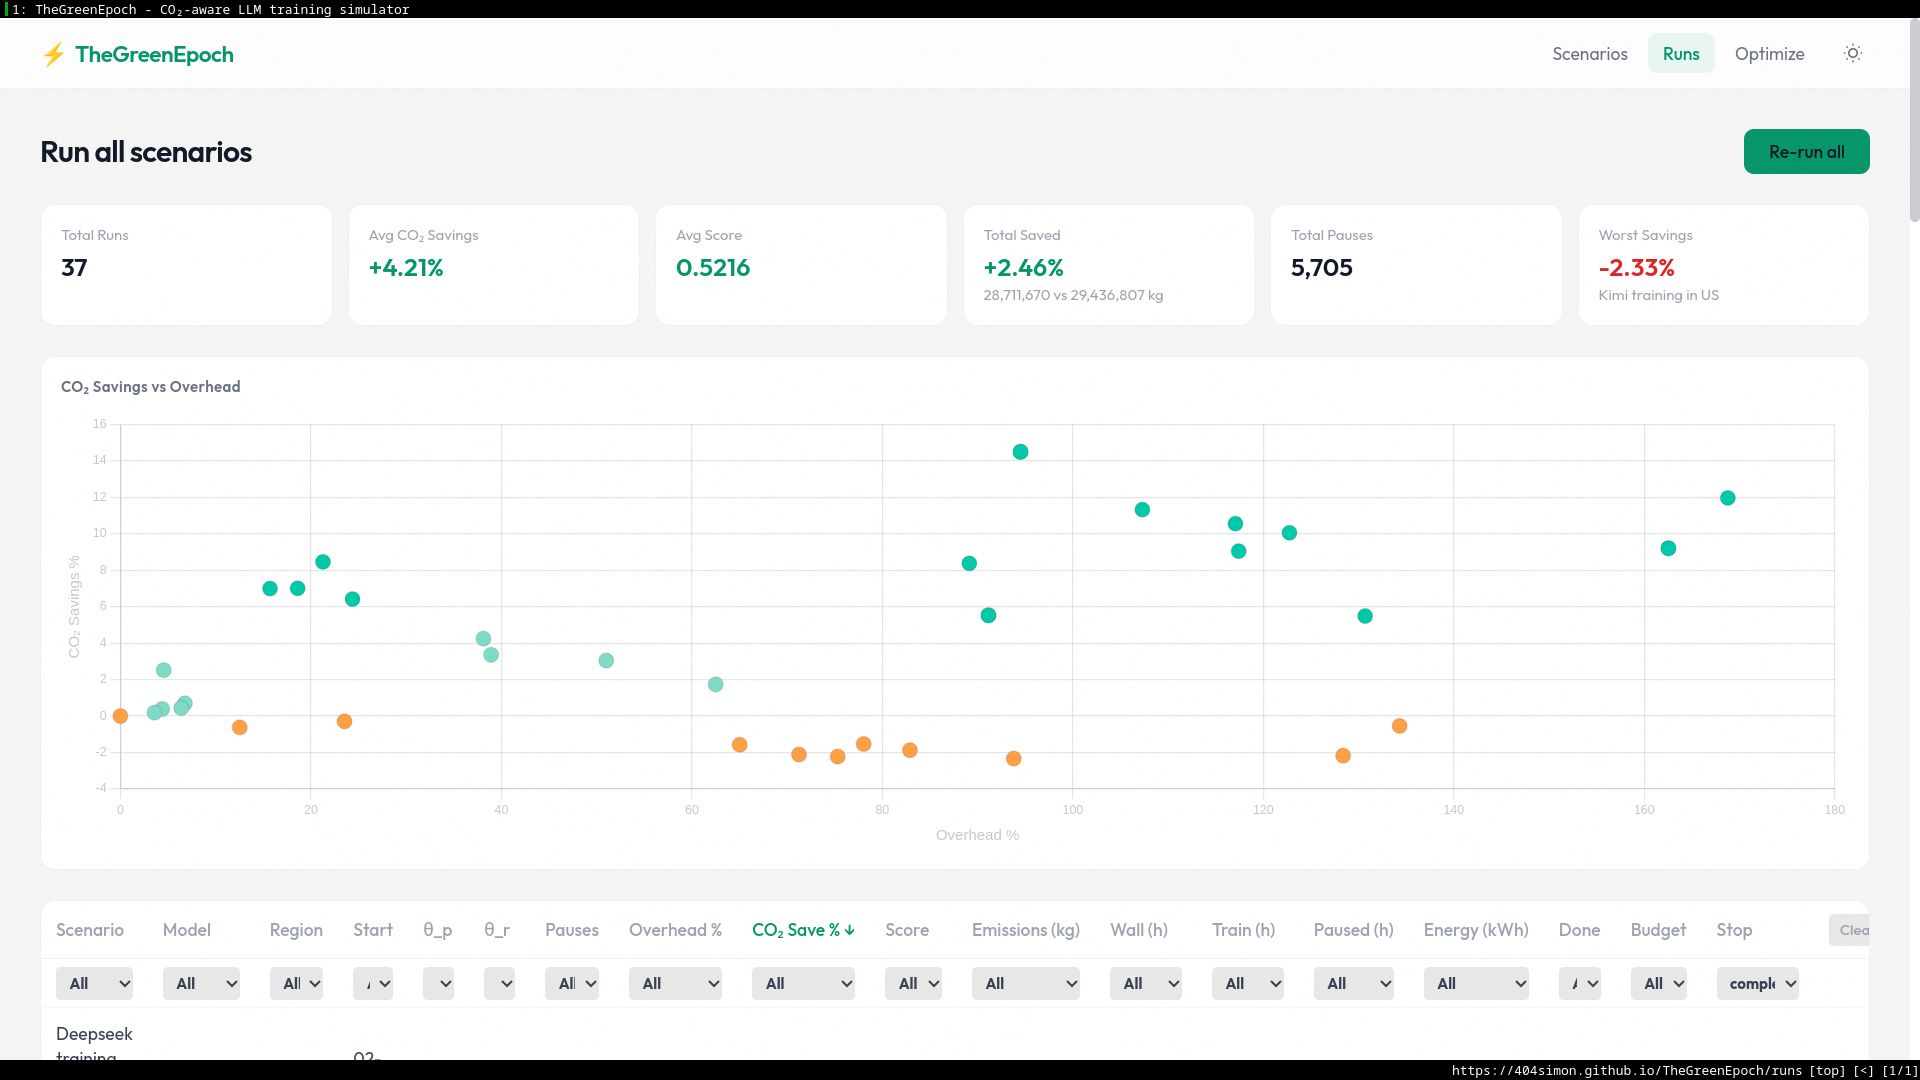
\includegraphics[width=\textwidth]{figures/screenshots/run_all_page_results_top_page}
  \caption{Batch run results view: scatter plot of CO$_2$ savings vs.\
  time overhead for all evaluated policies.}
  \label{fig:batch-scatter}
\end{figure}

\begin{figure}
  \centering
  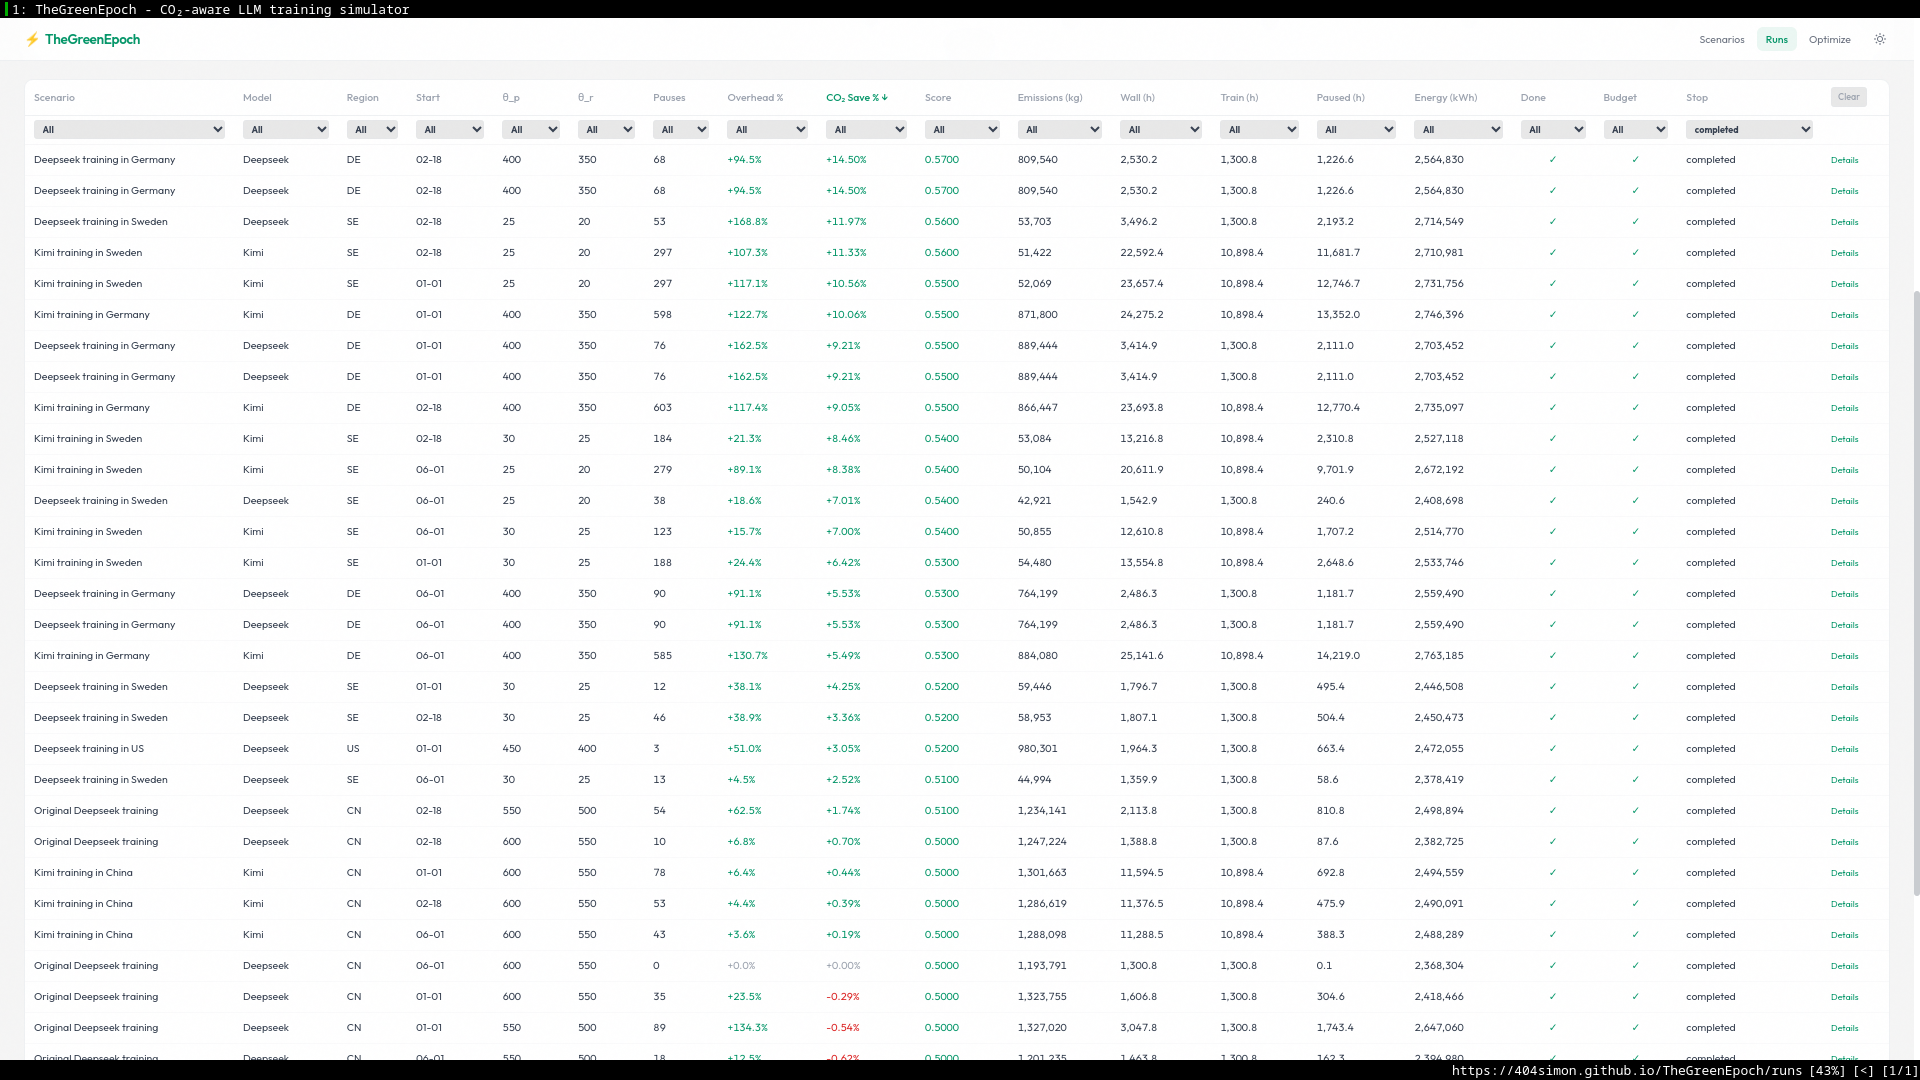
\includegraphics[width=\textwidth]{figures/screenshots/run_all_page_results_bottom_table}
  \caption{Batch run results table with sortable columns and detailed
  per-policy metrics.}
  \label{fig:batch-table}
\end{figure}

\section{Data Management}
\label{sec:data-management}

All data required for simulation is bundled with the application as static
JSON files:
\begin{itemize}
  \item \texttt{constants.json}: hardware constants (GPU power, power usage effectiveness,
    checkpoint overhead).
  \item \texttt{profiles.json}: training profiles for DeepSeek~V3 and
    Kimi~K2.
  \item \texttt{scenarios.json}: built-in default scenarios with preset
    parameters.
  \item \texttt{co2/*.json}: per-region, per-year CO$_2$ intensity time series
    at 5-minute resolution, pre-fetched from Electricity Maps.
\end{itemize}

User-created scenarios are persisted in the browser's localStorage.  The CO$_2$
data loader supports averaging multiple years into a representative timeline
and handles edge cases such as February 29 in leap years.

\section{CLI Tool}
\label{sec:cli}

In addition to the browser UI, the simulation and optimization engines are
exposed through a command-line interface using Commander.js.  The CLI supports
four commands:
\begin{itemize}
  \item \texttt{fetch}: download CO$_2$ intensity data from the Electricity
    Maps API for specified regions and date ranges.
  \item \texttt{run}: execute a batch of simulation scenarios and write
    results as CSV.
  \item \texttt{optimize}: run the adaptive grid-search optimizer from the
    command line and output the best policy configuration.
  \item \texttt{plot}: render optimization results as SVG charts for
    publication.
\end{itemize}

This dual-mode design (browser UI + CLI) ensures that the framework is useful
both for interactive exploration and for scripted, reproducible experiments.

%! TEX root = thesis.tex

\chapter{Experimental Setup}
\label{sec:experimental_setup}

\section{Models}
\label{sec:models}

We evaluate two state-of-the-art LLMs that represent the current frontier of
large-scale pretraining:

\begin{itemize}
  \item \textbf{DeepSeek~V3}~\cite{deepseek-ai_deepseek-v3_2024}: a 671B
    parameter mixture-of-experts model (37B active parameters per
    token), trained on 14.8T
    tokens using 2048 NVIDIA H800 GPUs, consuming 2.79M GPU-hours.
  \item \textbf{Kimi~K2}~\cite{kimi_team_kimi_2025}: a 1T parameter
    mixture-of-experts model
    (32B active), trained on 15.5T tokens with a minimum 256-GPU model-parallel
    group.
\end{itemize}

These two models differ substantially in scale: DeepSeek~V3 uses 8$\times$ more
GPUs, allowing us to examine how GPU count affects the savings-overhead
trade-off.

\section{Hardware Constants}
\label{sec:hardware-constants}

We use the following hardware parameters for all simulations:

\begin{table}
  \centering
  \caption{Hardware constants used in all simulations.}
  \label{tab:constants}
  \small
  \begin{tabular}{lr}
    \toprule
    Parameter & Value \\
    \midrule
    GPU training power & 700~W (NVIDIA H800) \\
    GPU idle power & 60~W \\
    Power usage effectiveness & 1.27 \\
    Checkpoint pause time & 148.8~s \\
    Checkpoint resume time & 0~s (async I/O) \\
    \bottomrule
  \end{tabular}
\end{table}

GPU training power is based on the NVIDIA H800 thermal design power
thermal design power~\cite{h800_specs}.  GPU idle power is estimated
from published hardware
measurements.  Power usage effectiveness is taken from DeepSeek's DGX
H800 infrastructure
report~\cite{jegham_hungry_2025}.  Checkpoint overhead is based on PyTorch
Distributed synchronous checkpoint measurements for a 7B model, with the
conservative assumption that checkpoint resume is overlapped with asynchronous
I/O~\cite{pytorch_checkpoint}.

\section{Regions and Data}
\label{sec:regions-data}

We evaluate five electricity grid regions: Germany (DE), Sweden (SE), Italy
(IT), the United States (US), and China (CN).  Carbon intensity data is
obtained from Electricity Maps at 5-minute resolution for the year 2025.
Table~\ref{tab:grid} in Chapter~\ref{sec:methodology} summarizes the grid
characteristics of each region.

\section{Optimizer Settings}
\label{sec:optimizer-settings}

All optimization runs use the following configuration:

\begin{table}
  \centering
  \caption{Adaptive optimizer configuration.}
  \label{tab:optimizer-config}
  \small
  \begin{tabular}{lr}
    \toprule
    Parameter & Value \\
    \midrule
    Grid resolution $N$ & 10 points per axis \\
    Maximum iterations $K$ & 10 \\
    Overhead budget $B$ & 200\% \\
    Shrink factor $s$ & 0.45 \\
    Trade-off parameter $\alpha$ & 1.0 (pure savings) \\
    $\theta_p^{\max}$ (Sweden) & 100~gCO$_2$eq/kWh \\
    $\theta_p^{\max}$ (others) & 800~gCO$_2$eq/kWh \\
    Start-date samples $D$ (optimized) & every 7th day \\
    Historical years & 2025 \\
    \bottomrule
  \end{tabular}
\end{table}

%! TEX root = thesis.tex

\chapter{Results}
\label{sec:results}

\section{Pareto Frontier Analysis}
\label{sec:pareto}

Figure~\ref{fig:pareto} presents the combined Pareto frontiers for both models
across all five regions.  Table~\ref{tab:best} reports the best-score
configurations with optimized start dates.

\begin{figure}
  \centering
  
\includegraphics[width=0.75\textwidth]{figures/savings_vs_overhead_all}
  \caption{Combined Pareto frontiers for DeepSeek~V3 and Kimi~K2 across five
  grid regions.  Each point is a feasible policy evaluated on 2025 5-minute
  intensity data.  Best-score points within 200\% overhead are highlighted.}
  \label{fig:pareto}
\end{figure}

For DeepSeek~V3, single-year savings range from 43.4\% (Germany, score 0.717)
to 6.2\% (China, score 0.531).  High-variability grids (Germany, Italy)
extend to high overheads (approaching 200\%) with correspondingly high
savings, while low-variance grids (US, CN) exhibit compressed frontiers
regardless of policy choice.

In high-variability grids, the frontier reflects abundant dirty intervals
worth avoiding.  Sweden plateaus earlier because the grid is so clean on
average that fewer dirty intervals exist.  The US and China show limited
temporal variation: pausing rarely finds a significantly cleaner interval than
the one it left.

For Kimi~K2, the same regional ordering holds at lower absolute savings
(Germany 27.5\%, score 0.637; China 2.4\%, score 0.512).  Larger GPU counts
amplify the benefit of avoiding dirty intervals, but the scaling is
sub-linear: DeepSeek~V3's up to 8$\times$ GPU advantage yields only 1.5 to
2.0$\times$ the relative savings, because checkpoint overhead also scales with
GPU count.

    \begin{table}
    \centering
    \caption{Best policy configurations per (model, region) with optimized
    start dates.  The hysteresis margin $\Delta_\theta = \theta_p - \theta_r$
    is at most 16~gCO$_2$eq/kWh across all combinations.}
    \label{tab:best}
    \small
    \begin{tabular}{llrrrrr}
      \toprule
      Model & Region & $\theta_p$ & $\theta_r$ & Savings & Overhead & Score \\
      \midrule
      DeepSeek~V3 & DE & 272 & 268 & 43.4\% & 174.3\% & 0.717 \\
      DeepSeek~V3 & IT & 246 & 231 & 32.7\% & 194.7\% & 0.663 \\
      DeepSeek~V3 & SE &  19 &  18 & 23.2\% & 106.3\% & 0.616 \\
      DeepSeek~V3 & US & 396 & 386 &  9.5\% & 115.7\% & 0.547 \\
      DeepSeek~V3 & CN & 528 & 512 &  6.2\% &  72.5\% & 0.531 \\
      \midrule
      Kimi~K2 & DE & 267 & 262 & 27.5\% & 199.4\% & 0.637 \\
      Kimi~K2 & IT & 283 & 271 & 16.6\% & 129.1\% & 0.583 \\
      Kimi~K2 & SE &  22 &  21 & 12.8\% & 115.4\% & 0.564 \\
      Kimi~K2 & US & 453 & 447 &  3.1\% &  22.2\% & 0.516 \\
      Kimi~K2 & CN & 537 & 522 &  2.4\% &  40.1\% & 0.512 \\
      \bottomrule
    \end{tabular}
\end{table}

The ranking of regions by savings potential (DE > IT > SE > US > CN) follows
the ranking by coefficient of variation.  Mean intensity plays a
secondary role: Sweden's high coefficient of variation is offset by its very low mean (23
gCO$_2$eq/kWh), limiting the absolute emissions available to avoid.

\section{Threshold Space and Hysteresis Margin}
\label{sec:threshold-space}

The central finding of this work emerges from the threshold space analysis.
Figure~\ref{fig:threshold} shows the pause vs.\ resume threshold plane for
DeepSeek~V3 in Germany, with color encoding the composite score.

\begin{figure}
  \centering
  
\includegraphics[width=0.75\textwidth]{figures/threshold_space_DeepSeek_V3_DE_0101}
  \caption{Pause vs.\ resume threshold for DeepSeek~V3 in Germany.  Color
  encodes composite score.  The diagonal $\theta_r = \theta_p$ marks
  zero-hysteresis policies.  High-scoring configurations cluster within a
  narrow margin, demonstrating that wide hysteresis margins are never
  Pareto-optimal.}
  \label{fig:threshold}
\end{figure}

Optimal hysteresis margins cluster near zero.  Across all 10 (model, region)
combinations, the best-score points satisfy the condition $\Delta_\theta \leq
16$~gCO$_2$eq/kWh, and in most cases $\Delta_\theta \leq
10$~gCO$_2$eq/kWh.  Zero-hysteresis policies ($\theta_r = \theta_p$) achieve
scores within 1--3\% of the optimum, confirming that a non-zero margin
provides marginal practical benefit.

Figure~\ref{fig:margin} confirms this pattern across the full policy set for
Kimi~K2.  Beyond $\Delta_\theta \approx 50$~gCO$_2$eq/kWh, wider margins
accumulate idle time and checkpoint overhead without proportional additional
savings.  A wide margin means training resumes only at very low intensities,
remaining paused through moderately clean intervals that could have been
exploited.

\begin{figure}
  \centering
  
\includegraphics[width=\textwidth]{figures/margin_vs_best_Kimi_K2}
  \caption{Composite score vs.\ hysteresis margin $\Delta_\theta$ for
  Kimi~K2.  Scores peak at $\Delta_\theta < 16$~gCO$_2$eq/kWh and plateau
  beyond $\Delta_\theta \approx 50$~gCO$_2$eq/kWh.  Zero-margin policies
  score within 1--3\% of the optimum.}
  \label{fig:margin}
\end{figure}

This finding is robust across two models and five regions, suggesting that a
near-zero margin is a fundamental property of the problem rather than an
artifact of our experimental settings.

\section{Start Date Sensitivity}
\label{sec:start-date}

Start date exerts a measurable but secondary influence on policy performance.
Across all (model, region) combinations, winter months (November to February)
are disproportionately represented among optimal start dates.  This reflects
lower grid carbon intensity during the heating season in many regions.

The effect ranges from approximately 20 percentage points of savings (Italy) to
under 2 percentage points (China), confirming that the hysteresis threshold
choice mostly, but not always, dominates start-date scheduling.

\section{Threshold Generalization Across Years}
\label{sec:threshold-generalization}

The best-scoring hysteresis threshold pairs for each model are not consistent across years.
Figure~\ref{fig:threshold-generalization} shows that the best-scoring thresholds for each model vary from year
to year, indicating that the optimal thresholds are sensitive to the specific carbon intensity
patterns of each year.  This suggests that a static threshold policy may not be optimal across
different years, and adaptive or year-specific threshold tuning could yield better performance
in terms of emissions savings and overhead management.

\begin{figure}
  \centering
  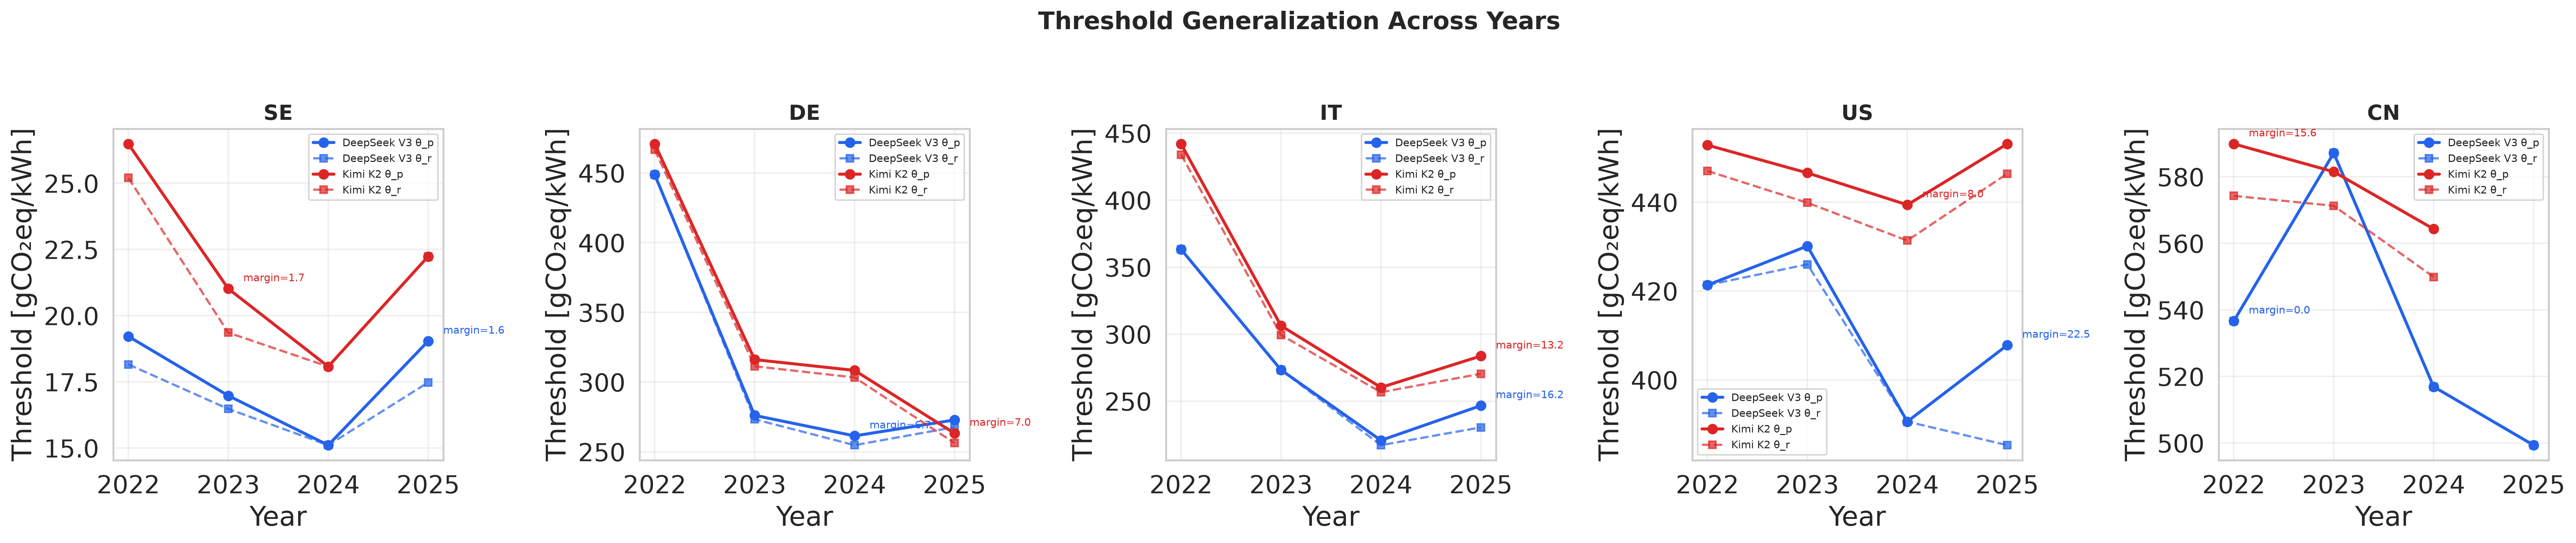
\includegraphics[width=1\textwidth]{figures/threshold_generalization}
  \caption{Threshold Generalization: Best scoring hysteresis threshold pairs for each model across the years from 2022 to 2025.}
  \label{fig:threshold-generalization}
\end{figure}


\section{Optimizer Convergence}
\label{sec:convergence}

The adaptive grid-search optimizer converges rapidly.  Figure~\ref{fig:convergence}
shows the score improvement across iterations for all (model, region)
combinations.  The score improves substantially between iterations 1 and 5,
plateaus by iteration 5 or 6, and subsequent iterations provide only marginal
refinement.

\begin{figure}
  \centering
  
\includegraphics[width=0.75\textwidth]{figures/score_vs_iteration_all}
  \caption{Optimizer convergence: composite score vs.\ iteration number for
  all (model, region) combinations.  Score plateaus by iteration 5--6 in all
  cases.}
  \label{fig:convergence}
\end{figure}

%! TEX root = thesis.tex

\chapter{Validation and Verification}
\label{sec:validation_verification}

\section{Validation}

Validation checks whether the simulation is an adequate representation of
real-world carbon-aware training for the study objectives.  It emphasizes
consistency with domain expectations rather than low-level code correctness.

\subsection{Structural Trade-off Behaviour}

The first validation checks the core trade-off between CO$_2$ savings and
training time overhead when varying the pause threshold $\theta_p$.  For fixed
region, start time, and model configuration, stricter thresholds (lower
$\theta_p$) should yield higher relative emission savings but also higher
wall-clock overhead.  The simulator is validated by confirming a monotone
trend in this trade-off and by inspecting the Pareto frontier for reasonable
shape and absence of pathological cases, such as negative savings for very
strict thresholds.


\subsection{Regional and Temporal Realism}

The third validation targets regional and temporal realism.  For each region
and year, an average grid carbon intensity is derived from the input time
series, and baseline emissions in a no-pause scenario should broadly follow
this ordering for fixed IT energy.  Additionally, under a chosen carbon-aware
pausing policy, regions or periods with high temporal variability in CO$_2$
intensity should exhibit greater potential savings than low-variance,
already-clean regions, albeit with more complex pause patterns.  Anomalous
results are checked against features of the underlying time series to ensure
they can be explained by specific training windows.


\section{Verification}

Verification ensures that the implementation follows the intended mathematical
model and uses the specified inputs and state updates correctly.  It is
carried out via targeted unit tests and synthetic test cases.

\subsection{Energy and Emissions Accounting}

The first verification step checks the energy and emissions accounting.  At
each time step, IT power, data center power, and incremental emissions are
computed from GPU counts, training or pause power, power usage effectiveness, and the CO$_2$
intensity.  The accumulated emissions over time, as well as baseline and
policy totals, are compared against analytical results in simple synthetic
scenarios.  Additionally, the KPI formulas for CO$_2$ savings percentage, time
overhead percentage, and the composite score are verified to match their
definitions for fixed numerical inputs.

\subsection{Pause/Resume Logic and Hysteresis}

The second verification step focuses on the pause/resume logic driven by the
pause threshold $\theta_p$ and hysteresis $\theta_r$.  A synthetic sequence of
CO$_2$ intensities is constructed to trigger known patterns of pausing and
resuming according to the specified hysteresis rule.  The simulated pause
state and pause count at each step are compared to the expected sequence,
ensuring that transitions only occur when the intensity crosses the configured
thresholds in the intended direction.

\subsection{Progress and Runtime Consistency}

The third verification step addresses consistency between training progress
and wall-clock time.  In non-paused steps, the progress fraction should
increase in proportion to the time step relative to the baseline training
time, while the elapsed wall time grows in every step.  In a no-pause
scenario, the simulation is expected to reach full progress exactly at the
baseline runtime within numerical tolerance.  In scenarios with pauses, the
simulated policy runtime is compared against the analytical expression
combining baseline time, total paused time, and per-pause checkpoint overhead.

\subsection{Unit Tests for KPI Functions}

Finally, KPI computations are tested in isolation through unit tests.  Fixed
values are supplied for baseline and policy emissions and runtimes, and the
functions computing CO$_2$ savings percentage, time overhead percentage, and
the composite score are checked against manually computed expected results.
This confirms that the KPI implementations are numerically correct,
independent of the rest of the simulation engine.


%! TEX root = thesis.tex

\chapter{Conclusion}
\label{sec:conclusion}

We have presented a simulation framework and adaptive grid-search optimizer
for carbon-aware LLM training via hysteresis-based pausing.  The framework
replays historical grid carbon intensity data through a discrete-event
simulator, and the optimizer efficiently searches the three-dimensional policy
space of pause threshold, resume threshold, and start date.  Across two
state-of-the-art models (DeepSeek~V3 and Kimi~K2) and five grid regions with
diverse variability profiles, we establish systematic Pareto frontiers for
this problem.

The central finding is that hysteresis provides diminishing returns: the
optimal policy uses a narrow or zero margin ($\Delta_\theta \leq
16$~gCO$_2$eq/kWh) in every region and model.  Wide hysteresis margins waste
time and checkpoint overhead without proportional savings.  Carbon-aware
pausing can reduce operational emissions by up to 43\% in high-variability
grids at the cost of up to 200\% wall-clock overhead.  In low-variance grids,
savings fall below 10\%, and alternative mitigation strategies such as
geo-distributed training should be considered.

Our implementation as a fully client-side browser application demonstrates
that carbon-aware training simulation and optimization can be made accessible
to researchers and practitioners without specialized infrastructure.  The
application provides an interactive live simulator, a batch run dashboard,
and an adaptive optimization page with real-time 3D visualization of the
policy space.

\section{Limitations}

Our simulation assumes perfect foresight: policies are evaluated on historical
data rather than forecasted future intensity.  A real deployment would require
forecasting, introducing prediction error.  We use a fixed checkpoint overhead
derived from a 7B model; real overhead depends on model size and storage
bandwidth and may scale with the number of model parameters.  GPU idle power
is an estimate, and actual values vary across hardware generations and data
center configurations.  Finally, this work considers single-site training;
geo-distributed training could compound savings by adding spatial flexibility.

\section{Future Work}

Three directions are particularly promising for future work:
\begin{enumerate}
  \item \textbf{Forecast-based policies.}  Replace historical replay with
    predictive carbon intensity forecasts (e.g.\ using ECMWF or local grid
    operator data) to enable real-time deployment.
  \item \textbf{Multi-job scheduling.}  Extend the framework to optimize across
    multiple training jobs sharing a GPU cluster, balancing carbon savings with
    fairness and throughput.
  \item \textbf{Embodied carbon awareness.}  Incorporate manufacturing
    emissions to ensure that operational savings from pausing are not
    outweighed by amortized hardware production costs.
\end{enumerate}

All simulation code and data are available as open source at
\url{https://github.com/404simon/TheGreenEpoch}.


\cleardoublepage{}

\appendix

% \include{chapters/95-appendix}
% \chapter*{\glossarytitlename}
\addcontentsline{toc}{chapter}{\glossarytitlename}

\begin{acronym}[ABCDEFGHIJK]
    \acro{API}{Application Programming Interface}
    \acro{CLI}{Command-Line Interface}
    \acro{CO2}{Carbon Dioxide}
    \acro{FAU}{Friedrich-Alexander-Universit\"at Erlangen-N\"urnberg}
    \acro{GPU}{Graphics Processing Unit}
    \acro{LLM}{Large Language Model}
    \acro{SOTA}{State of the Art}
\end{acronym}

\clearpage

% \printnomenclature
\addcontentsline{toc}{chapter}{Nomenclature}
\clearpage

% Add list of figures.
\listoffigures
\addcontentsline{toc}{chapter}{List of Figures}
\clearpage
% Add list of tables.
\listoftables
\addcontentsline{toc}{chapter}{List of Tables}
\clearpage
% Add bibliography.
\sloppy
\printbibliography
\addcontentsline{toc}{chapter}{Bibliography}

\end{document}
